\documentclass[symbols]{fei}
\usepackage[utf8]{inputenc}
\usepackage{amsmath}
\usepackage{graphicx}
\usepackage[table]{xcolor} % Ativa o suporte de cores para tabelas
\usepackage{float}
\usepackage{tabularx} % Para tabelas que se ajustam ao texto
\usepackage{array} % Para melhores opções de coluna
\usepackage{setspace} % Para espaçamento
\usepackage{lipsum} % Para texto de exemplo, se necessário
\usepackage[backend=biber]{biblatex}
\addbibresource{referencias.bib}
\newsubfloat{figure}

\renewcommand\thesection{\arabic{section}}
\renewcommand\thesubsection{\thesection.\arabic{subsection}}
\renewcommand\thesubsubsection{\thesubsection.\arabic{subsubsection}}

\begin{document}

%\begin{titlepage} % Início da página de título
\vspace*{\fill} % Espaço no topo (ajusta para centralizar verticalmente)
\begin{center}
%\setstretch{1.5} % Define o espaçamento entre linhas para 1.5
{\LARGE \textbf{Técnicas de Análise de Dados Aplicadas a Biopotenciais no Treinamento de Pilotos do Motosport}} % Título principal em fonte grande
\end{center}
\vspace{6cm}% Adiciona 2 cm de espaço vertical 
Orientador: Prof. Dr. Wellington Cássio Pinheiro \\
Departamento: Engenharia Mecânica \\
Candidato: Mateus Marana Assuena\\
N°:22.123.026-1 
\vspace{2cm} \\ % Adiciona 2 cm de espaço vertical
Início: abril/2025 \\
Previsão conclusão:  março/2026
\vspace*{\fill} % Espaço no fundo (ajusta para centralizar verticalmente)
%\end{titlepage}

\newpage

\begin{center}
    \textbf{RESUMO}
\end{center}

Este projeto visa investigar o efeito da fadiga muscular nos pilotos de \textit{motorsport} utilizando técnicas de análise de dados 
aplicada a biopotenciais. O foco será a implementação de algoritimos de inteligência artificial e \textit{machine learning} para 
relacionar a performance e a exposição prolongada a exercícios físicos intensos com a fadiga muscular. Dados preliminares foram coletados com voluntários das 
equipes do BAJA e Fórmula da FEI realizando exercícios na academia com ênfase grupos musculares flexores e extersores de punho, apontados pelos pilotos
como intensamente demandados durante as corridas. 
O projeto utilizará a eletromiografia de superfície (sEMG) para entender a atividade elétrica muscular durante as etapas do percurso e como a fadiga afeta o desempenho do atleta. 
Espera-se que, por meio de técnicas de aprendizagem de máquina, as análises realizadas identifiquem padrões relevantes, permitindo a mitigação dos impactos da fadiga nos atletas do automobilismo e gerando \textit{insights}
sobre a preparação dos pilotos.\\
\\
\textbf{Palavras-chave:} motorsport; análise de dados; clusterização; classificação; inteligência artificial; machine learning; fadiga muscular; eletromiografia.

\newpage

\section{Revisão de Literatura}
\subsection{Introdução e contextualização}

O \textit{motorsport} é uma das modalidades esportivas mais populares do mundo \cite{ferguson2015_optimizing}. Competições como Fórmula 1 e NASCAR 
atraem telespectadores de todo o mundo, contando com uma audiência de 5 milhões de pessoas por evento \cite{ferguson2015_optimizing}. Por envolver 
velocidade, é uma modalidade de alta intensidade que exige dos pilotos boa resistência física e capacidade cognitiva para 
praticá-lo \cite{ferguson2007_reactivity}

Com base na Fédération Internationale de l'Automobile (FIA), a industria do \textit{motorsport} gera um volume bruto anual estimado 
em cerca de € 159,2 bilhões e emprega aproximadamente 1,5 milhão de trabalhadores pagos em todo o mundo \cite{fia_impact_2021}. Nos 
Estados Unidos, estudo da Performance Racing Industry (PRI) indicou um impacto econômico superior a US\$ 69,2 bilhões anuais e emprega 
mais de 318 mil pessoas nos diversos elos da cadeia do automobilismo \cite{pri_study_2025}.

De acordo com o estudo conduzido por Hoyes e Collins (2018), os pilotos de automobilismo relatam qual é o 
principal requisito físico necessário para o desempenho ideal durante as corridas, segundo suas experiências \cite{fittorace}. 
Os autores destacam que, embora força e estabilidade também sejam importantes, a resistência cardiorrespiratória é considerada pelos 
próprios atletas como o fator mais determinante para suportar as demandas fisiológicas das competições.

Estudos mostram que sessões prolongadas de condução levam à fadiga neuromuscular, reduzindo a precisão motora e 
a eficiência de resposta muscular \cite{lecocq2020neuromuscular}. A análise de biopotenciais e sinais inerciais 
se destaca como um conjunto de técnicas que podem ser utilizadas para compreender melhor a biomecânica dos pilotos e permitir o 
entendimento  de como a fadiga muscular afeta o desempenho na prática do esporte. 

A fadiga muscular é definida como uma diminuição transitória da capacidade de realizar ações físicas, ou seja, uma redução momentânea no desempenho 
muscular mesmo antes da falha completa \cite{enoka2007_muscle_fatigue}. Esse fenômeno influencia diretamente a função muscular, uma vez que altera o 
recrutamento das unidades motoras e as propriedades de condução das fibras, modificando a amplitude e a frequência dos sinais eletromiográficos durante o esforço prolongado.

O objetivo principal deste estudo é aplicar métodos de aprendizado de máquina e inteligência artificial, na análise da fadiga muscular 
dos pilotos. Por meio desses modelos, pretende-se identificar padrões relevantes nos sinais de sEMG e inerciais que indiquem estados de 
fadiga, provendo análise que possam orientar os profissionais da saúde na elaboração de programas de treinamento mais personalizadose 
estratégias de competição que reduzam perdas de desempenho relacionadas a esforço muscular excessivo, otimizando tanto os treinos quanto 
o rendimento em competições.

\subsection{Biomecânica dos Pilotos}

Biomecânica é o estudo do movimento das coisas vivas \cite{knudson}, utilizando-a podemos entender melhor como o corpo humano e, 
neste estudo , os atletas do motorsport, se utilizam de forças de contração muscular e torques articulares na produção de movimentos e 
como esses movimentos se coordenam para a execução de uma tarefa. Em particular, o estudo da biomecânica é  uma ferramenta para entender 
e aperfeiçoar o desempenho humano \cite{neuromechanics}.  

Considerando que o automobilismo é um esporte de alta intensidade, a ativação muscular e neurológica exigida para controlar o veículo e realizar 
tomadas rápidas de decisão pode comprometer o sistema motor dos pilotos. Em situações de uso prolongado, há risco de fadiga localizada, que reduz 
a precisão contrátil e prejudica o desempenho competitivo \cite{mills2025_forearm_activity}.  

A fadiga é um fenômeno multifatorial que resulta em redução temporária da capacidade funcional do sistema nervoso e da força muscular 
\cite{fatigueimpact}. Sendo vista em várias atividades que necessitam de esforço do indivíduo, ela pode acarretar em um séries de 
fatores que, em períodos mais longos, resultam em problemas de saúde. Alguns de seus efeitos registrados são o cansaço, lapsos 
cognitivos e a perda de performance a longo prazo \cite{fatigueaviation}. A fadiga muscular é caracterizada pela redução 
prolongada da capacidade de gerar força, sendo associada ao aumento da amplitude da sEMG e à transição da alta para a baixa 
frequência \cite{thelastarticle}.

Um estudo realizado mostra que as voltas inicias dos competidores são na maioria das vezes as melhores enquanto as últimas são 
comprometidas. Credita-se esse compromentimento ao desgaste físico e mental acumulado \cite{learningcurves}. 
Para mitigar esses efeitos, estratégias como pausas para recuperação muscular e sessões de treino mais curtas, seguidas de 
análises detalhadas dos erros, podem ser eficazes \cite{learningcurves}. Essa abordagem visa preservar o desempenho durante períodos mais longos e 
reduzir a incidência de fadiga severa.
 
Estudo de Delmuns Carvajal et al. (2023) apontou que os membros superiores dos pilotos de kart estão sujeitos a variações significativas 
na atividade muscular devido a fatores como o desenho da pista, a lateralidade do piloto e a presença de sistemas de embreagem. 
Por exemplo, curvas realizadas no lado dominante do piloto resultam em maior ativação muscular, enquanto a troca de marchas acrescenta 
esforço adicional, alterando os padrões de movimento. 

Os membros superiores estendem-se da cintura escapular, composta por escápula, clavícula e articulação glenoumeral, até a mão, englobando ombro, 
braço e antebraço \cite{kenhub_upper}. O braço contém o úmero e músculos dos compartimentos anterior (bíceps, coracobraquial e braquial) e posterior (tríceps), 
enquanto o antebraço é composto pelos ossos rádio e ulna, e pelos músculos dos compartimentos flexor e extensor, incluindo flexor radial do carpo, 
flexor ulnar do carpo, pronador redondo, supinador, extensores dos dedos e extensores do carpo sendo inervado pelos nervos mediano, ulnar e radial. A mão apresenta ossos 
carpais, metacarpos e falanges, com músculos que garantem precisão e força \cite{kenhub_hand}.

Os membros inferiores vão da cintura pélvica (ilíaco, ísquio e púbis) até o pé, compreendendo coxa e perna \cite{kenhub_lower}. A coxa abriga o fêmur e 
músculos dos grupos quadríceps e isquiotibiais; a perna contém tíbia e fíbula, com músculos gastrocnêmio, sóleo e tibial anterior; e o pé é formado por ossos do 
tarso, metatarso e falanges, sustentados por músculos responsáveis pela estabilidade e propulsão \cite{ncbi_footmuscles}.

As articulações dos membros superiores incluem a glenoumeral, cotovelo, rádio-ulnares, 
punho e interfalângicas, que permitem movimentos como flexão, extensão e rotação \cite{pubmed_joints}. Durante a condução, 
atuam no controle do volante, trocas de marcha e estabilização do tronco, com amplitudes médias de 14°–54° no ombro, 35°–72° 
no cotovelo e 34°–23° no punho \cite{monash_upper}, além de alta ativação muscular em manobras rápidas \cite{pubmed_upper_activation}. A operação dos 
pedais exige forte ativação dos isquiotibiais, gastrocnêmio e reto femoral, com torques maiores no quadril, seguidos de joelho e 
tornozelo \cite{mdpi_lower}. Em frenagens de emergência, motoristas idosos exibem maior ativação do sóleo e atraso no reto femoral, sugerindo maior 
demanda muscular \cite{pubmed_lower_reaction}.

\subsection{Biopotenciais e Eletromiografia}

Biopotenciais são sinais elétricos gerados por processos fisiológicos que ocorrem dentro do corpo. São produzidos a  partir da 
atividade eletroquímica de uma célula excitável. Quando estimulada, uma célula excitável gera um potencial de ação, a qual é a 
fonte essencial dos processos biopotenciais no corpo \cite{macy2025}.

O sEMG capta a atividade elétrica das fibras musculares durante contrações voluntárias ou involuntárias, 
por meio de eletrodos colocados sobre a pele. Ele permite estimar parâmetros como intensidade de ativação e recrutamento de unidades motoras, 
servindo como ferramenta para investigar o comportamento funcional dos músculos durante diferentes tipos de esforço \cite{farina2016_biophysics, merletti2023_current_sEMG}.  
A EMG de superfície, em particular, é amplamente empregada na avaliação da fadiga muscular e do controle motor, desempenhando papel essencial em contextos clínicos e 
esportivos \cite{deLuca2016_surfaceEMG}.

A aplicação desses métodos nos diferentes domínios proporciona uma compreensão mais aprofundada dos processos fisiológicos envolvidos 
na fadiga muscular, contribuindo significativamente para melhorar o desempenho em atividades de longa duração.\cite{thelastarticle}

\subsection{IMUs}
Os sensores IMU (Unidade de Medição Inercial) são amplamente utilizados para capturar e analisar o movimento humano em diversas 
aplicações, incluindo biomecânica e reabilitação. Esses dispositivos combinam acelerômetros, giroscópios e, em alguns casos, magnetômetro.
Sua precisão na análise do movimento tem sido demonstrada em estudos recentes, destacando sua importância na avaliação clínica e na 
validação de desempenho em diversas tarefas motoras \cite{meng2023,favata2024}.

\begin{itemize}
    \item \textbf{Acelerômetro}:
    Mede a aceleração linear em três eixos (X, Y e Z), sendo essencial para identificar os impactos e forças aplicadas nos membros superiores durante 
    curvas e frenagens. Essas informações ajudam a entender como as forças G afetam o corpo do piloto em diferentes situações de corrida.

    \item \textbf{Giroscópio}:
    Registra a velocidade angular, captando rotações e inclinações do tronco e dos membros superiores. Esse sensor será útil 
    para analisar a dinâmica de manobras rápidas, como mudanças de direção e estabilização após curvas.

    \item \textbf{Magnetômetro}:
    Detecta a orientação em relação ao campo magnético terrestre, permitindo um monitoramento preciso da direção do corpo e 
    da postura do piloto no espaço tridimensional.
\end{itemize}

Os sensores Trigno Avanti™ incluem uma unidade de medição inercial (IMU) integrada com nove graus de liberdade (9-DOF). 
Esses sensores permitem registrar as medidas incerciais de forma sincronizada aos sinais EMG \cite{delsys_trigno_manual}. 
As faixas típicas de operação variam de ±2 g a ±16 g para o acelerômetro e ±250°/s a ±2000°/s para o giroscópio, garantindo alta 
precisão na análise de movimento e postura dos participantes \cite{delsys_trigno_manual}.

\begin{table}[H]
\centering
\caption{Especificações técnicas dos sensores utilizados no sistema \textit{Trigno™ Wireless EMG} (Delsys Inc.)}
\label{tab:trigno_specs}
\begin{tabular}{|p{5cm}|p{9cm}|}
\hline
\textbf{Parâmetro} & \textbf{Especificação Técnica} \\ \hline
\textbf{Fabricante / Modelo} & Delsys Inc., Boston, EUA — Sistema \textit{Trigno™ Wireless EMG} \\ \hline
\textbf{Tipo de sensor} & Eletromiografia de superfície (EMG) sem fio, com opção de módulo inercial (IMU) integrado \\ \hline
\textbf{Faixa de frequência (banda passante)} & 20 -- 450 Hz (filtro analógico passa-faixa interno Butterworth de 4ª ordem) \\ \hline
\textbf{Taxa de amostragem} & 2000 Hz por canal (configuração padrão para EMG); até 4000 Hz em modo de alta resolução \\ \hline
\textbf{Resolução do conversor A/D} & 16 bits \\ \hline
\textbf{Faixa de entrada} & ±11 mV (ajustável até ±22 mV) \\ \hline
\textbf{Ruído de fundo} & $\leq$ 750 nV RMS \\ \hline
\textbf{Latência de transmissão} & Inferior a 500 µs (transmissão digital sem fio de baixa latência) \\ \hline
\textbf{Precisão temporal entre sensores} & $\pm$1 µs de defasagem máxima entre canais sincronizados \\ \hline
\textbf{Distância operacional} & Até 40 m (linha de visada direta) \\ \hline
\textbf{Autonomia da bateria} & Aproximadamente 8 horas de operação contínua \\ \hline
\textbf{Dimensões / Massa} & 37 × 26 × 15 mm / 14 g \\ \hline
\textbf{Material dos eletrodos} & Prata pura (99,99 \%) com encapsulamento em polímero selado \\ \hline
\textbf{IMU integrada (opcional)} & Acelerômetro triaxial (±16 g), giroscópio (±2000 °/s) e magnetômetro (±4900 µT) \\ \hline
\textbf{Interface de software} & Compatível com \textit{EMGworks®}, \textit{Trigno SDK}, e integração via MATLAB®/Python® \\ \hline
\textbf{Ambiente operacional} & 5–40 °C, umidade relativa $\leq$ 80 \% (sem condensação) \\ \hline
\end{tabular}
\end{table}

\subsection{Aplicação da RMS na Análise de Fadiga no Motorsport}

A \textit{Root Mean Square} (RMS) é uma métrica estatística utilizada para mensurar a magnitude efetiva de sinais variáveis, 
especialmente em contextos biomédicos e de engenharia em que sua fórmula, para um sinal discreto $x[n]$ com $N$ amostras, é dada por:  

\begin{equation}
\text{RMS} = \sqrt{\frac{1}{N} \sum_{n=1}^{N} x[n]^2}
\end{equation}

essa medida permite representar a intensidade média de um sinal oscilatório sendo amplamente utilizada na análise de sinais eletromiográficos por sua capacidade de 
refletir a amplitude e a variabilidade do sinal em função da atividade muscular \cite{deluca1997use}. 
À medida que a fadiga se instala, observa-se uma tendência de aumento na amplitude do sinal elétrico captado em razão da necessidade de maior 
recrutamento de unidades motoras para compensar a perda de eficiência muscular \cite{gandevia2001}.

Adicionalmente, ao segmentar o sinal em janelas de duração fixa, pode-se calcular a RMS de cada trecho, obtendo uma análise dinâmica da 
fadiga ao longo do tempo \cite{merletti2004electromyography}.

\subsection{Média da Amplitude da Variação (MAV) na Análise de Fadiga no Motorsport}

A Média da Amplitude da Variação (MAV) é um parâmetro utilizado na análise de sinais eletromiográficos por sua simplicidade 
de cálculo e eficácia na detecção de alterações relacionadas à fadiga muscular. A MAV é definida como a média dos valores absolutos da 
amplitude do sinal em uma janela de tempo, permitindo uma quantificação direta da atividade elétrica do músculo. Sua fórmula pode ser 
expressa como:

\[
MAV = \frac{1}{N} \sum_{i=1}^{N} |x_i|
\]

em que \(x_i\) representa a i-ésima amostra do sinal e \(N\) é o número total de amostras dentro da janela de análise \cite{phinyomark2012feature}.

Durante períodos prolongados de esforço físico, observa-se um aumento da amplitude do sinal EMG associado à necessidade de recrutamento 
de um maior número de unidades motoras para manter o desempenho, seguido por uma redução conforme a fadiga muscular 
se instala \cite{deluca1997use}.

Além disso, a integração da MAV com outras métricas, como a RMS, potencializa a análise multidimensional da fadiga \cite{merletti2004electromyography}. Essa abordagem permite 
identificar períodos críticos de declínio do desempenho do piloto, 
fornecendo informações relevantes para estratégias de treinamento, ergonomia e ajuste da carga de trabalho durante a competição \cite{phinyomark2012feature,deluca1997use}.

\subsection{Espectrograma e Análise da Fadiga em Motorsport}

O espectrograma é uma ferramenta utilizada na análise de sinais biológicos, permitindo a visualização conjunta das 
componentes de frequência ao longo do tempo em um sinal. Ele é obtido por meio de \textit{Short-Time Fourier Transform}, que divide o sinal em 
janelas temporais e aplica a transformada de Fourier em cada segmento, resultando em uma representação tempo-frequência e sua formulação matemática pode ser descrita como:

\begin{equation}
X(\tau, \omega) = \sum_{n=-\infty}^{\infty} x[n] \, w[n - \tau] \, e^{-j \omega n}
\end{equation}

em que \(x[n]\) é o sinal original, \(w[n]\) é a janela de análise, \(\tau\) representa o deslocamento temporal e \(\omega\) a 
frequência angular \cite{allen1977short}. Essa abordagem permite identificar como a energia do sinal se distribui ao longo do tempo 
em diferentes bandas de frequência.

Na análise da fadiga muscular, o espectrograma aplicado a sinais EMG permite observar alterações na distribuição espectral ao longo do tempo. Durante o progresso da fadiga, 
é comum um deslocamento da energia para bandas de baixa frequência, refletindo aumento de potência nessas regiões e redução da variabilidade 
espectral \cite{puce2021_spectral, rodrigues2022_emg_processing}
   

\section{Materiais e Métodos}
\subsection{Métodos}

Primeiramente, foi realizado um aprofundamento da revisão de literatura aqui apresentada, com o objetivo de aprimorar os conhecimentos 
em biomecânica dos pilotos, eletromiografia e machine learning na análise de dados. De forma concomitante, foi realizada a 
familiarização com tópicos da biomecânica computacional importantes à execução da pesquisa.

A coleta de dados foi realizada na academia do campus com os pilotos do Fómula FEI e BAJA, utilizando de exercícios que simulam a 
pilotagem de carros de corrida, focando nos músculos presentes no antebraço. A eletromiografia de superfície foi empregada para 
monitorar a ativação muscular dos pilotos durante o esforço físico. O processo de coleta foi dividido em etapas, a fim de identificar 
padrões distintos de fadiga e desempenho muscular.

A atividade eletromiográfica foi registrada por meio do sistema \textit{Trigno™ Wireless EMG} (Delsys Inc., Boston, EUA), 
composto por sensores sem fio, posicionados sobre os músculos Braquiorradial, Extensor do Carpo Ulnar, 
Extensor dos Dedos e Palmar Longo. A fixação dos sensores seguiu as recomendações do fabricante, respeitando o 
alinhamento das fibras musculares e os procedimentos de preparação da pele, a 
fim de garantir baixa impedância e máxima qualidade do sinal. Entre as séries de coleta, foi adotado um intervalo 
de recuperação de 10 minutos para minimizar os efeitos de fadiga residual. 

O protocolo experimental foi repetido em três dias distintos, com intervalo mínimo de 24 horas entre as sessões, 
permitindo a análise da variabilidade interdiária e o controle de efeitos adaptativos. Os sinais EMG foram transmitidos 
em tempo real para a unidade base do sistema, armazenados em ambiente computacional seguro e posteriormente processados 
para normalização, segmentação e extração de parâmetros relevantes à análise de fadiga muscular.

\subsection{Utilização do Sistema Trigno na Coleta de Dados para Análise de Fadiga Muscular}

A coleta dos sinais elétricos foi realizada por meio do sistema \textit{Trigno™ Wireless EMG} (Delsys Inc., Boston, EUA). 
O sistema é composto por sensores sem fio miniaturizados, dotados de eletrodos de prata (99,99 \%) encapsulados em corpo selado e 
resistente, com área de contato típica de 5 × 1 mm \cite{trigno_manual}. Os sinais são transmitidos via rádio a uma unidade 
base receptora, com alcance de até 40 m em condições ideais de visada direta \cite{trigno_specs}.

Os sensores EMG do sistema Trigno operam com taxa de amostragem de 2 000 Hz por canal, o que permite a captura precisa de 
componentes de alta frequência do sinal mioelétrico e evita aliasing durante a análise espectral \cite{trigno_specs, trigno_userguide}. 
A faixa de frequência efetiva (banda passante) é de 20 Hz a 450 Hz, adequada para a maioria dos estudos de ativação muscular 
voluntária \cite{trigno_manual}. A resolução de conversão analógico-digital é de 16 bits, com faixa de entrada 
típica de ±11 mV a ±22 mV, ajustável conforme a configuração experimental \cite{trigno_personal_manual}.

A comunicação entre sensores e unidade base ocorre por transmissão digital sem fio de baixa latência (inferior a 500 µs), 
garantindo a sincronização precisa entre múltiplos canais de aquisição \cite{trigno_specs}.

Cada sensor é alimentado por uma bateria interna recarregável de íons de lítio, com autonomia de operação contínua de até 8 horas. 
O carregamento é realizado por meio de estações dedicadas, permitindo a rotação dos sensores entre sessões experimentais sem perda de 
produtividade \cite{trigno_specs}.

\subsection{Procedimento de Coleta de Dados}

A coleta de dados foi conduzida com o objetivo de registrar a atividade eletromiográfica (EMG) dos músculos do antebraço durante 
exercícios de resistência muscular. O experimento foi realizado em ambiente controlado, garantindo condições adequadas de temperatura, 
iluminação e ausência de interferências eletromagnéticas.

\subsubsection{Preparação do participante}

Inicialmente, o piloto foi preparado para o experimento por meio de limpeza e depilação da região de interesse, reduzindo a impedância 
elétrica da pele e garantindo a qualidade dos sinais. Em seguida, foram identificados e demarcados os pontos anatômicos correspondentes 
aos músculos:
\begin{itemize}
    \item \textbf{Braquiorradial},
    \item \textbf{Extensor do Carpo Ulnar},
    \item \textbf{Extensor dos Dedos}, e
    \item \textbf{Palmar Longo}.
\end{itemize}

Os sensores do sistema Trigno foram fixados sobre os ventres musculares, respeitando o alinhamento das fibras e seguindo as 
recomendações do fabricante quanto à orientação e distância entre eletrodos. Cada sensor foi calibrado individualmente antes 
do início da coleta, assegurando a estabilidade e fidelidade do sinal durante todo o processo.

\subsubsection{Execução do exercício}

O protocolo experimental consistiu em três séries do exercício de rosca punho, realizadas até a falha muscular voluntária, 
com foco na ativação dos músculos extensores e flexores do antebraço. Entre cada série, foi concedido um intervalo 
de 10 minutos de descanso, a fim de permitir a recuperação parcial e minimizar a influência da fadiga residual.  

Durante a primeira sessão, observou-se que a primeira repetição apresentou maior duração, uma vez que o participante demorou mais 
tempo para atingir a falha muscular.

\subsubsection{Sessões experimentais}
O protocolo completo foi repetido em três dias distintos, com intervalo de 24 horas entre as sessões. Essa estratégia permitiu avaliar a variabilidade interdiária e controlar possíveis efeitos de aprendizado, adaptação neuromuscular ou fadiga cumulativa.

\begin{figure}[H]
    \centering
    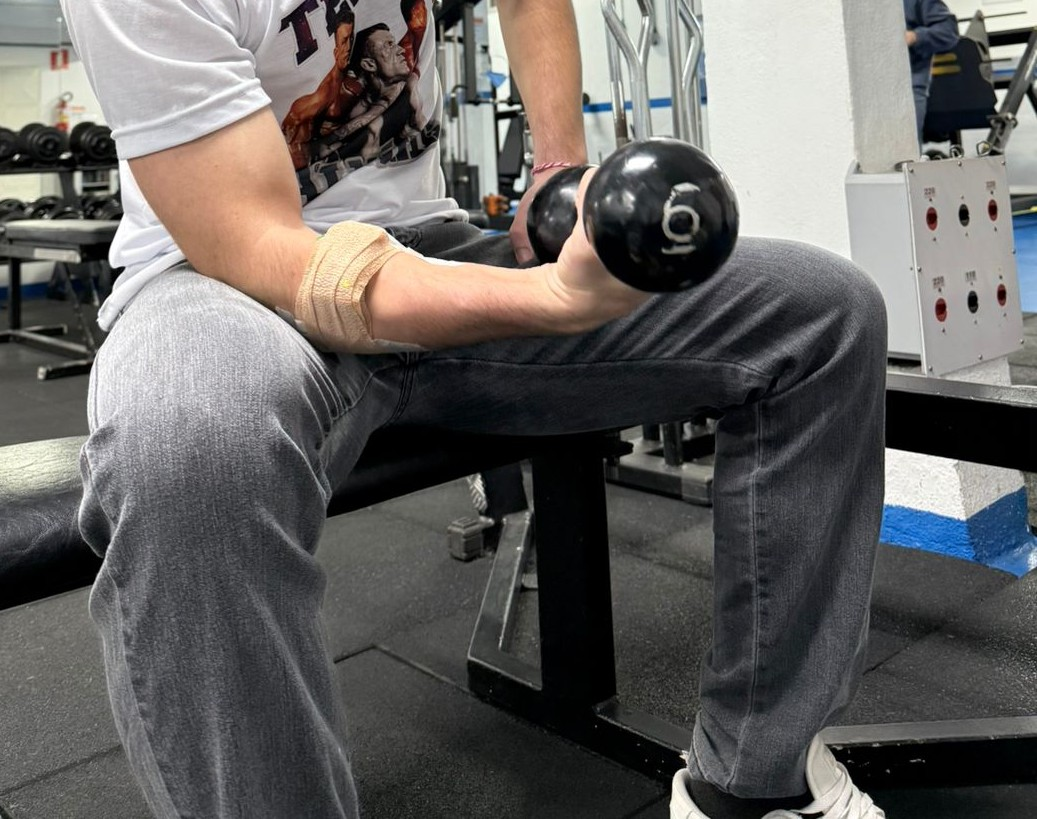
\includegraphics[width=0.7\textwidth]{images/Exercicio_Rosca_Punho.jpeg}
    \caption{Simulação do exercício de rosca punho realizado durante a primeira coleta na academia. O participante manteve o antebraço apoiado e realizou o movimento de flexão e extensão do punho até a falha muscular.}
    \label{fig:exercicio_rosca_punho}
\end{figure}

\begin{figure}[H]
    \centering
    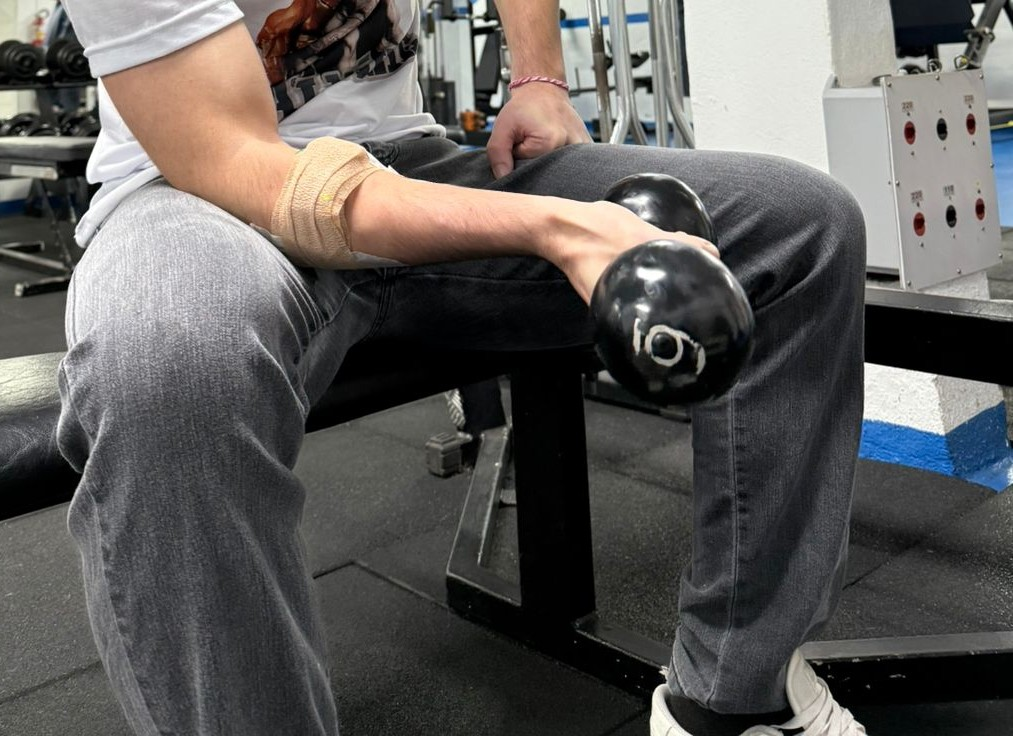
\includegraphics[width=0.7\textwidth]{images/Exercicio_Rosca_Punho(1).jpeg}
    \caption{Simulação do exercício de rosca punho realizado durante a primeira coleta na academia. O participante manteve o antebraço apoiado e realizou o movimento de flexão e extensão do punho até a falha muscular.}
    \label{fig:exercicio_rosca_punho}
\end{figure}

O \textit{Trigno Wireless EMG} demonstrou excelente desempenho na captação dos sinais mioelétricos, oferecendo uma ferramenta 
robusta e precisa para o estudo da fadiga muscular em condições controladas, sem comprometer a liberdade de movimento do participante..

\subsection{Pipeline Computacional e Modelo Baseado em PINN}

Após a etapa de aquisição do EMG, foi desenvolvido um pipeline computacional responsável pela extração de 
características, construção de um índice fisiológico de fadiga e treinamento de um modelo baseado em PINNs. Esse pipeline foi estruturado com o 
objetivo de transformar o sinal bruto em uma representação temporal contínua e interpretável da fadiga muscular.

\subsubsection{Extração de características do sinal EMG}

Os sinais EMG foram segmentados em janelas temporais de 5 segundos, com o objetivo de reduzir a 
variabilidade instantânea do sinal e capturar padrões estatísticos mais estáveis. 

No domínio temporal, foram extraídas as métricas RMS, MAV e ZCR. 
O RMS foi utilizado como estimador da potência efetiva do sinal EMG, sendo empregado na literatura como indicador do nível de ativação muscular. O MAV 
foi calculado para representar a amplitude média do sinal, fornecendo uma medida complementar da intensidade da atividade 
eletromiográfica. Já o ZCR foi utilizado para quantificar a taxa de cruzamentos por zero, refletindo a complexidade e o 
conteúdo de frequência do sinal, parâmetros que tendem a sofrer alterações durante o processo de fadiga muscular.

No domínio da frequência, aplicou-se a Transformada Rápida de Fourier (FFT) após o janelamento do sinal por meio da janela de Hamming, 
adotada para minimizar efeitos de \textit{leakage} espectral decorrentes da análise de segmentos finitos do sinal. Em seguida, foi realizada uma 
suavização gaussiana do espectro, visando reduzir flutuações locais e aumentar a robustez da extração das características espectrais.

A partir do espectro suavizado foram obtidas a Frequência Média (MNF), a Frequência Mediana (MDF) e o Desvio Espectral. 
A MNF e a MDF foram selecionadas por serem reconhecidas como importantes indicadores de fadiga muscular, uma vez que o 
processo de fadiga está associado ao deslocamento do conteúdo espectral do 
EMG para faixas de menor frequência. O desvio espectral foi 
utilizado para caracterizar a dispersão da energia ao 
longo do espectro de frequências, permitindo avaliar alterações na distribuição espectral do sinal.

Adicionalmente, foi empregada a análise por espectrograma para incorporar informações 
tempo-frequência ao processo de caracterização dos sinais. A partir dessa 
representação foram extraídas a energia espectral média e a frequência dominante. A 
energia espectral foi utilizada como medida da intensidade global da atividade 
muscular ao longo do tempo, enquanto a frequência dominante permitiu identificar a faixa espectral com maior concentração de energia em cada janela analisada.

A seleção dessas características foi fundamentada 
em sua relevância fisiológica e em sua ampla utilização 
em estudos de análise de fadiga muscular baseada em 
eletromiografia, possibilitando uma representação 
abrangente das alterações de amplitude e frequência que ocorrem durante o esforço prolongado.

\subsubsection{Construção do índice fisiológico de fadiga}

Devido à inexistência de um marcador direto e quantitativo capaz de representar instantaneamente o nível de fadiga muscular a partir dos 
sinais eletromiográficos, foi desenvolvido um índice fisiológico de fadiga utilizado como referência para o 
treinamento supervisionado do modelo proposto. Esse índice tem como objetivo sintetizar, em uma única variável contínua, as 
alterações fisiológicas observadas nas diferentes características extraídas do sinal EMG ao longo do exercício.

Inicialmente, todas as features foram normalizadas para o intervalo, visando eliminar diferenças 
de escala entre as variáveis e garantir contribuições comparáveis na composição do índice. Em seguida, 
foi realizada uma combinação ponderada das características temporais e espectrais, considerando o comportamento 
fisiológico esperado de cada métrica durante o processo de fadiga muscular.

As variáveis RMS, MAV e energia espectral foram incorporadas diretamente ao índice por apresentarem 
tendência de aumento com a progressão da fadiga. Por outro lado, as métricas ZCR, MNF, MDF e frequência dominante foram invertidas, uma vez que normalmente 
apresentam redução ao longo do esforço muscular prolongado em decorrência do deslocamento do conteúdo espectral para faixas de menor frequência.

O índice final foi obtido por meio da média ponderada das contribuições 
provenientes dos diferentes músculos monitorados, permitindo uma 
representação global do estado fisiológico do antebraço. Posteriormente, 
foi aplicada uma suavização temporal baseada em média móvel, com o objetivo 
de reduzir oscilações locais e aumentar a continuidade temporal do sinal resultante.

Dessa forma, o índice fisiológico de fadiga 
fornece uma aproximação contínua da evolução da 
fadiga muscular ao longo do exercício, servindo como variável 
alvo para o treinamento da PINN.


\subsubsection{Arquitetura da PINN}

O modelo desenvolvido consiste em uma rede neural artificial totalmente 
conectada, cuja entrada é composta pelas características temporais e espectrais extraídas dos sinais 
eletromiográficos, acrescidas da informação temporal normalizada. A inclusão explícita do tempo como variável de 
entrada permite que o modelo aprenda não apenas relações estáticas entre as features e o estado de fadiga, mas também a 
dinâmica temporal associada à evolução do fenômeno ao longo do exercício.

A arquitetura adotada foi composta por três camadas ocultas contendo 128, 128 e 64 neurônios, respectivamente, todas utilizando função de ativação
Tangente Hiperbólica (\textit{Tanh}). A escolha dessa função de ativação foi motivada por sua suavidade e 
diferenciabilidade contínua em todo o domínio, características importantes em PINNs, uma vez que o processo de treinamento 
envolve o cálculo de derivadas de primeira e segunda ordem da saída da rede em relação às variáveis de entrada.

Diferentemente de arquiteturas convencionais voltadas exclusivamente para ajuste de dados, a PINN busca incorporar informações 
relacionadas ao comportamento físico esperado do sistema analisado. Dessa forma, a utilização de funções suaves 
contribui para a obtenção de aproximações contínuas e fisiologicamente plausíveis da evolução da fadiga muscular.

A saída da rede consiste em um único valor escalar para cada instante analisado, representando a estimativa 
contínua do índice de fadiga muscular ao longo do tempo.

\subsubsection{Função de perda e processo de treinamento}

O treinamento da PINN foi realizado por meio de uma função de perda composta por termos orientados tanto pelos dados experimentais 
quanto por restrições associadas ao comportamento esperado da fadiga muscular. Essa abordagem permite que o modelo não apenas 
reproduza os padrões observados nos dados, mas também respeite características físicas inerentes ao fenômeno estudado.

O primeiro componente da função de perda, denominado \textit{(Ldata)}, corresponde ao Erro Quadrático Médio (MSE) entre as predições da rede e o 
índice de fadiga previamente construído. Esse termo é responsável por garantir que a saída da rede permaneça consistente com as 
informações extraídas dos sinais eletromiográficos.

Além do ajuste aos dados, foram incorporadas restrições físicas por meio da análise das derivadas da 
saída da rede em relação ao tempo normalizado. O termo \textit{(Lmono)} foi definido para 
penalizar valores negativos da derivada temporal da fadiga, impondo a hipótese de que, durante o exercício contínuo, a fadiga 
apresenta comportamento predominantemente não decrescente. Dessa forma, o modelo é desencorajado a 
produzir reduções abruptas ou fisiologicamente improváveis no índice de fadiga ao longo do tempo.

Adicionalmente, foi introduzido o termo de regularização \textit{(Lreg)}, baseado na 
segunda derivada temporal da saída da rede. Esse componente atua como um mecanismo de 
suavização, penalizando variações excessivamente bruscas na inclinação da curva prevista e 
favorecendo a obtenção de trajetórias temporalmente contínuas e compatíveis com a evolução gradual da fadiga muscular observada experimentalmente.

A função de perda total utilizada no treinamento pode ser expressa por:

\[
	Ltotal = Ldata + \lambda mono * Lmono + \lambda reg * Lreg
\]

em que $\lambda$mono e $\lambda$reg representam coeficientes de ponderação responsáveis por 
controlar a influência das restrições físicas sobre o processo de otimização. Dessa forma, a minimização da 
função de perda busca simultaneamente maximizar a aderência aos dados experimentais e garantir coerência nas estimativas produzidas pela rede.

O treinamento foi realizado utilizando o algoritmo de otimização Adam, amplamente 
empregado em aplicações de aprendizado profundo devido à sua capacidade de adaptação 
dinâmica das taxas de atualização dos parâmetros. Foi adotada uma taxa de aprendizado 
inicial, complementada por um mecanismo de ajuste. Esse procedimento reduz automaticamente a taxa de 
aprendizado quando a função de perda apresenta estagnação por um 
número pré-definido de épocas, favorecendo a convergência do modelo e evitando oscilações durante as etapas finais do treinamento.


\subsubsection{Interpretação do modelo PINN}

A PINN desenvolvida neste trabalho busca aprender uma função contínua capaz de relacionar as características temporais e espectrais extraídas dos 
sinais eletromiográficos com a evolução do estado de fadiga muscular ao longo do exercício. Diferentemente de 
abordagens orientadas por dados, a incorporação de restrições físicas ao processo de treinamento permite que o modelo produza 
estimativas consistentes não apenas com os dados experimentais, mas também com o comportamento fisiológico esperado do fenômeno analisado.

Nesse contexto, as restrições impostas à função de perda favorecem a obtenção de curvas de fadiga suaves e coerentes, 
reduzindo oscilações artificiais e penalizando comportamentos incompatíveis com a progressão da fadiga muscular. Como resultado, 
o modelo combina a capacidade de aprendizado das redes neurais profundas com conhecimentos prévios sobre a 
dinâmica do sistema biológico, contribuindo para uma representação mais robusta, interpretável e plausível da evolução da fadiga ao longo do tempo.

\section{Resultados}

Nesta seção são apresentados os resultados obtidos a partir da análise dos sinais de EMG coletados durante o protocolo experimental. As análises incluem 
representações no domínio tempo-frequência, métricas fisiológicas extraídas dos sinais e a modelagem da fadiga por meio da PINN.

\subsection{Análise no Domínio Tempo-Frequência}

Os espectrogramas permitem observar a evolução das componentes de frequência ao longo do tempo para cada grupo muscular analisado.

\begin{figure}[H]
    \centering
    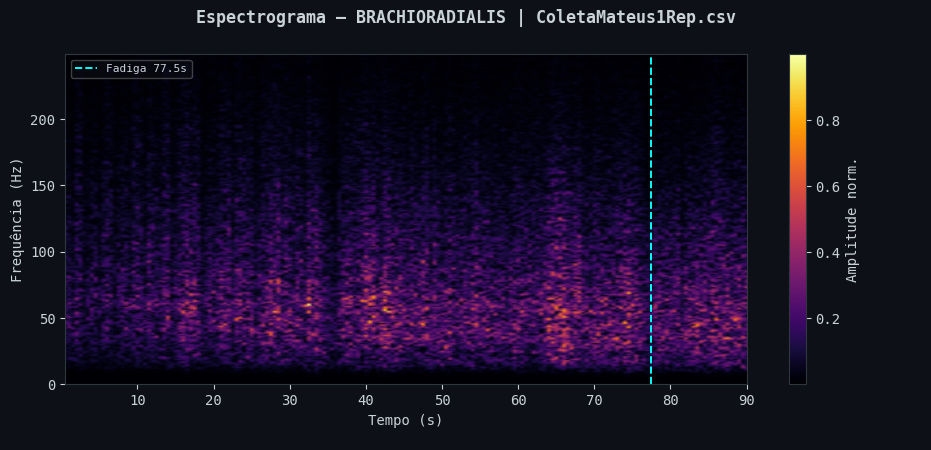
\includegraphics[width=0.9\linewidth]{images/Espec_1.png}
    \caption{Espectrograma do músculo Extensor Digitorium. A linha tracejada indica o instante estimado de fadiga.}
    \label{fig:spec_ext_dig}
\end{figure}

No músculo Extensor Digitorium (Figura \ref{fig:spec_ext_dig}), observa-se uma maior concentração de energia nas faixas de baixa frequência ao longo do tempo. 
Esse comportamento é consistente com a literatura, que associa a fadiga muscular à redução da frequência mediana do sinal EMG. Além disso, 
há aumento da intensidade do sinal nas regiões finais do exercício, indicando maior recrutamento de unidades motoras.

\begin{figure}[H]
    \centering
    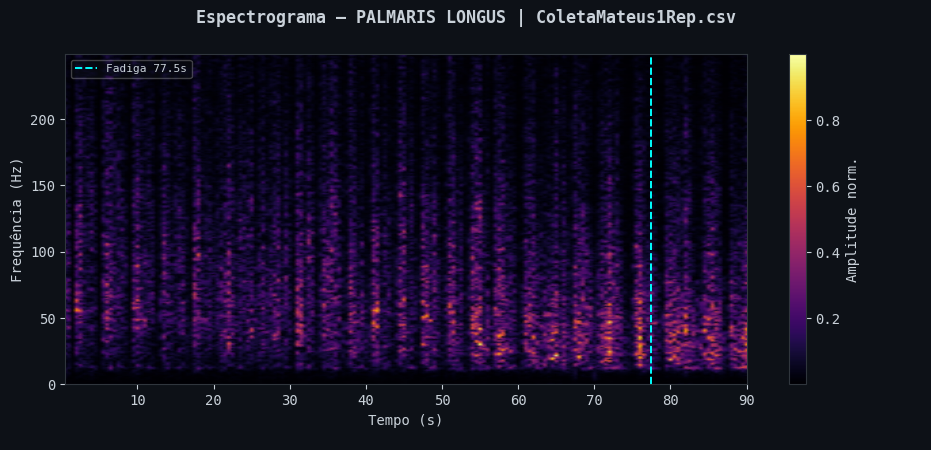
\includegraphics[width=0.9\linewidth]{images/Espec_3.png}
    \caption{Espectrograma do músculo Palmaris Longus.}
    \label{fig:spec_palmar}
\end{figure}

Para o músculo Palmaris Longus (Figura \ref{fig:spec_palmar}), observa-se comportamento semelhante, com aumento progressivo da energia em baixas 
frequências e maior densidade espectral conforme o esforço se prolonga. Esse padrão sugere fadiga localizada, com perda de eficiência muscular.

\begin{figure}[H]
    \centering
    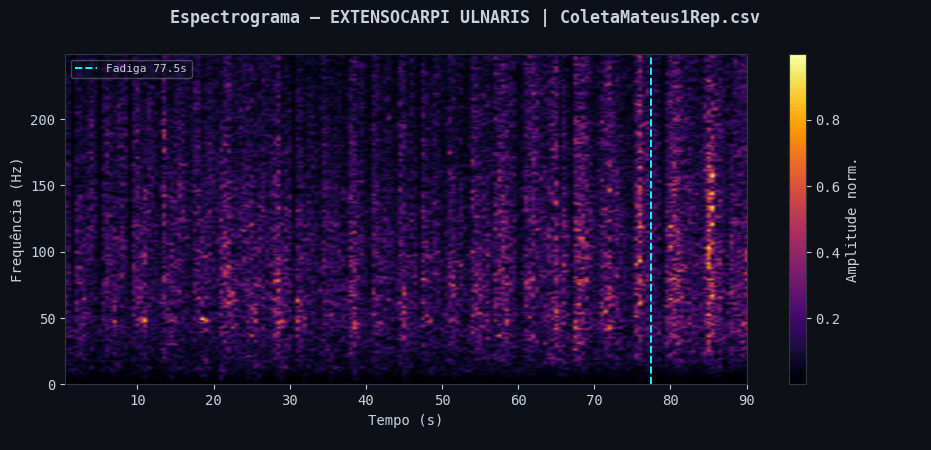
\includegraphics[width=0.9\linewidth]{images/Espec_2.png}
    \caption{Espectrograma do músculo Extensor Carpi Ulnaris.}
    \label{fig:spec_ext_carp}
\end{figure}

No Extensor Carpi Ulnaris (Figura \ref{fig:spec_ext_carp}), o espectrograma apresenta maior dispersão de energia ao longo das frequências,
indicando um comportamento mais instável do recrutamento muscular. Ainda assim, é possível observar tendência de deslocamento espectral para 
frequências mais baixas próximo ao instante de fadiga.

De forma geral, os espectrogramas evidenciam o fenômeno clássico da fadiga muscular: aumento da amplitude do sinal e deslocamento espectral para baixas frequências.

\subsection{Métricas Fisiológicas Extraídas}

\begin{figure}[H]
    \centering
    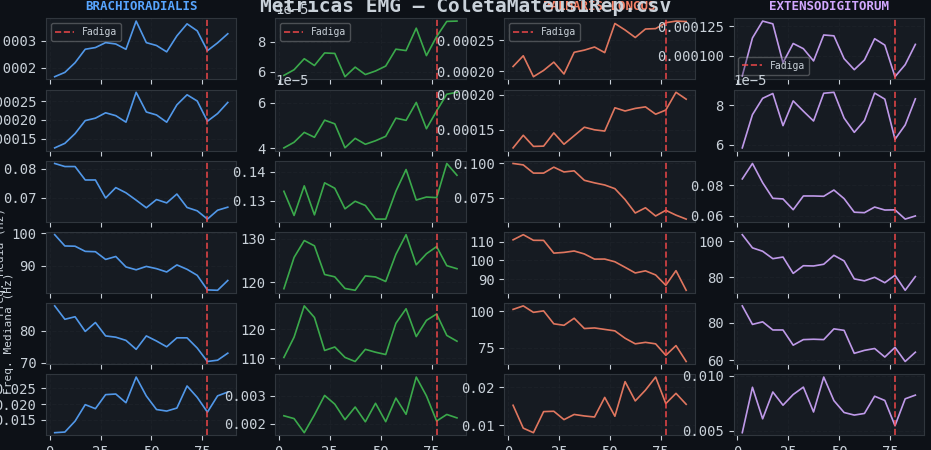
\includegraphics[width=\linewidth]{images/Metricas.png}
    \caption{Evolução temporal das métricas extraídas dos sinais EMG para os diferentes músculos analisados.}
    \label{fig:metricas}
\end{figure}

A Figura \ref{fig:metricas} apresenta a evolução temporal de diferentes métricas extraídas dos sinais EMG, incluindo RMS, MAV, frequência mediana e 
outras características estatísticas.

Observa-se que:

\begin{itemize}
    \item A \textbf{RMS} apresenta tendência de aumento ao longo do tempo, refletindo maior ativação muscular para compensar a fadiga;
    
    \item A \textbf{MAV} segue comportamento semelhante, indicando aumento da atividade elétrica média;
    
    \item A \textbf{frequência mediana} apresenta tendência de queda, caracterizando o deslocamento espectral associado à fadiga;
    
    \item Há maior variabilidade nas métricas nos instantes finais do exercício, sugerindo instabilidade neuromuscular.
\end{itemize}

Esses resultados estão alinhados com o comportamento esperado em condições de fadiga muscular progressiva.

\subsection{Modelagem da Fadiga com PINN}

\begin{figure}[H]
    \centering
    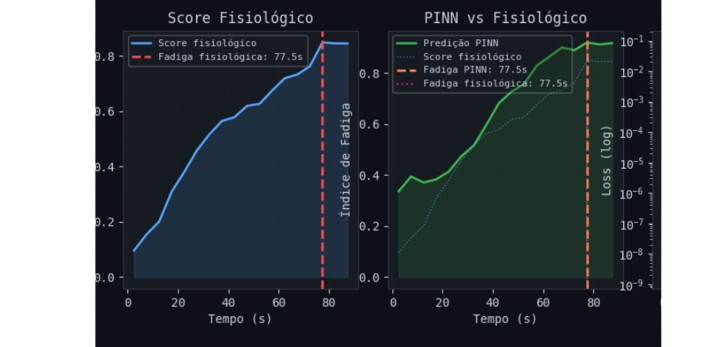
\includegraphics[width=0.45\linewidth]{images/Design_sem_nome-removebg-preview.png}
    \caption{(Esquerda) Evolução do score fisiológico de fadiga. (Direita) Comparação entre a predição da PINN e o score fisiológico.}
    \label{fig:pinn}
\end{figure}

A Figura \ref{fig:pinn} apresenta a evolução do score fisiológico de fadiga e sua modelagem por meio da PINN.

O \textbf{score fisiológico} apresenta crescimento monotônico ao longo do tempo, refletindo o acúmulo progressivo de fadiga durante o exercício. O ponto de fadiga 
foi identificado aproximadamente em 77.5 segundos, conforme indicado pela linha tracejada.

A \textbf{PINN} demonstrou alta capacidade de modelar a dinâmica da fadiga, acompanhando de forma consistente a tendência do score fisiológico. Observa-se que:

\begin{itemize}
    \item A rede captura corretamente o comportamento crescente da fadiga;
    
    \item Há boa aproximação entre predição e dado real, especialmente nas regiões intermediárias do sinal;
    
    \item Pequenas discrepâncias podem ser observadas nos instantes iniciais e finais, possivelmente associadas a ruídos ou variações fisiológicas individuais.
\end{itemize}

Esses resultados indicam que a abordagem baseada em PINN é promissora para modelagem de fenômenos fisiológicos complexos, como a fadiga muscular.

\subsection{Síntese dos Resultados}

De forma geral, os resultados demonstram que:

\begin{itemize}
    \item Os sinais EMG apresentam padrões claros de fadiga, tanto no domínio do tempo quanto da frequência;
    
    \item As métricas extraídas são consistentes com a literatura fisiológica;
    
    \item A PINN foi capaz de modelar a evolução da fadiga com boa precisão;
    
    \item A integração entre análise de sinais e inteligência artificial permite identificar padrões relevantes para o desempenho muscular.
\end{itemize}

Esses achados reforçam o potencial do uso de técnicas de análise de dados e aprendizado de máquina na avaliação da fadiga muscular em pilotos de motorsport.

\printbibliography

\end{document}
